% =============================================================================
% Title:        Flow Controller Wiring
% Author:       Nathaniel Thomas
% Affiliation:  Texas A&M University, Department of Nuclear Engineering
% Email:        nathaniel@tamu.edu
% Date Created: 3/7/2026
% Version:      1.0
%
% Description:
%   A .tex file outlining the wiring for the Aalborg flow controllers used
%   to control the flow of gases in the FLiNaK purifier.
%
% =============================================================================

\section{Flow Controller Wiring}

There are three Aalborg GFC17s used to control the flow of \ch{H2}, \ch{HF},
and \ch{Ar} in this system. The flow controllers were rewired to reduce the male
DB15 connectors coming
from the Aalborg connectors to DB9 connectors before being
wired into the NI USB-6353. Refer to \Cref{fig: DB15 to DB9 connector
diagram} and \Cref{tab: flow controller wiring}. The reduction to a
9-pin connector was
done because a number of connectors on the flow controllers were not used
in this system, such as the 4-20 mA control signals. \par

\begin{enumerate}
  \item The power supply for the flow controllers were consolidated
    into a single 24V, 2A
    power supply. In addition, the power for the HF sensor was also
    supplied from the same
    power supply.
  \item Each flow controller draws \SI{650}{\milli\ampere} at
    \SI{24}{\volt}. The HF sensor draws a
    maximum of \SI{1.4}{\watt}. At \SI{24}{\volt}, this becomes a
    draw of $\SI{1.4}{\watt} / \SI{24}{\volt}  = \SI{0.058}{\milli\ampere}$.
    The power supply has a maximum limit of \SI{2}{\ampere}. With three
    flow controllers and the HF sensor, the total draw from the power supply
    is \SI{1950.06}{\milli\ampere}.
\end{enumerate}

\begin{figure}[H]
  \centering
  % =============================================================================
% Title:        Flow Controller DB15 to DB9 Connector Diagram
% Author:       Nathaniel Thomas
% Affiliation:  Texas A&M University, Department of Nuclear Engineering
% Email:        nathaniel@tamu.edu
% Date Created: 3/7/2026
% Version:      1.0
%
% Description:
%   A colored wiring diagram of the FLiNaK purifier flow controllers.
%   This diagram shows the wire connections for the DB15 female to DB9 female
%   connecting cables used to connect the Aalborg flow controllers to the
%   NI USB-6353 that controls the purifier.
%
% =============================================================================

\begin{circuitikz}
    \node[draw, minimum width=1.5cm, minimum height=4.5cm] (A) {DB9};
    % Right DB9 connector
    \node[draw, minimum width=1.5cm, minimum height=7.5cm, right=6cm
    of A] (B) {DB15};

    % Left connector pins
    \foreach \i [evaluate=\i as \y using {2 - 0.5*(\i-1)}] in {1,...,9}
    {
      \node[circle, draw, inner sep=1pt] (L\i) at (1.5,\y) {};
      \node[left] at (L\i) {\i};
    }
    \node[circle, draw, inner sep=1pt] (LGND) at (0,-3) {};
    \node[above] at (LGND) {GND};

    % Right connector pins
    \foreach \i [evaluate=\i as \y using {3.5 - 0.5*(\i-1)}] in {1,...,15}
    {
      \node[circle, draw, inner sep=1pt] (R\i) at (6,\y) {};
      \node[right] at (R\i) {\i};
    }
    \node[circle, draw, inner sep=1pt] (RGND) at (7.5,-4.5) {};
    \node[above] at (RGND) {GND};

    \newcommand{\pinconnect}[3]{%
      % #1 = DB9 pin, #2 = DB15 pin, #3 = color
      \draw[#3, thick] (L#1) -- (R#2);
    }

    \pinconnect{1}{1}{orange}
    \pinconnect{2}{2}{yellow}
    \pinconnect{3}{4}{green}
    \pinconnect{4}{8}{blue}
    \pinconnect{5}{7}{red}
    \pinconnect{6}{10}{violet}
    \pinconnect{7}{11}{darkgray}
    \pinconnect{8}{12}{lightgray}
    \pinconnect{9}{5}{black}
    \draw[brown, thick] (LGND) -| (L9);
    \draw[brown, thick] (RGND) -| (R15);
    \draw[brown, thick] (R15.west) -- ++(-1,0) |- (R5.west);
    \draw[brown, thick] (R3.west) -- ++(-1,0) |- (R5.west);
\end{circuitikz}

  \caption{A wiring diagram showing the DB15 to DB9 wiring connections for the
    gas flow controllers used in the system. Grounding wires are
    shown in brown, and ground is tied to the negative pole of the
  24V power supply.}
  \label{fig: DB15 to DB9 connector diagram}
\end{figure}

\begin{table}[H]
  \centering
  \begin{tabular}{llll}
    DB9 pin number & DB15 pin number & Wire color & Purpose \\
    \hline
    1 & 1 & \color{orange}orange & 0 to 5 Vdc flow signal common \\
    2 & 2 & \color{yellow}yellow & 0 to 5 Vdc flow signal output \\
    3 & 4 & \color{green}green & Open (Purge) \\
    4 & 8 & \color{blue}blue & Remote setpoint input \\
    5 & 7 & \color{red}red & +24 Vdc power supply \\
    6 & 10 & \color{violet}purple & Remote setpoint common \\
    7 & 11 & \color{darkgray}gray & +5 Vdc reference output for
    remote setpoint \\
    8 & 12 & \color{lightgray}white & Valve off control \\
    9 & 5 & \color{black}black & Common, power supply \\
    \hline
    GND & 3 & \color{brown}brown & Common \\
    - & 6 & \color{black}none & (unassigned) \\
    - & 9 & \color{black}none & 4-20 mA (-) flow signal return \\
    - & 13 & \color{black}none & Auxiliary +24 Vdc \\
    - & 14 & \color{black}none & 4-20 mA (+) flow signal output \\
    - & 15 & \color{brown}brown & Chassis ground \\
    \hline
  \end{tabular}
  \caption{Table of wiring for DB15 to DB9 connectors for Aalborg
  GFC17 mass flow controllers. Refer to \Cref{sec:aalborg pinout} for details.}
  \label{tab: flow controller wiring}
\end{table}

Refer to \Cref{fig: gfc db9} for an image of the wired 9-pin connector.
Refer to \Cref{fig: gfc db15} for an image of the wired 15-pin connector.

\begin{figure}[H]
  \centering
  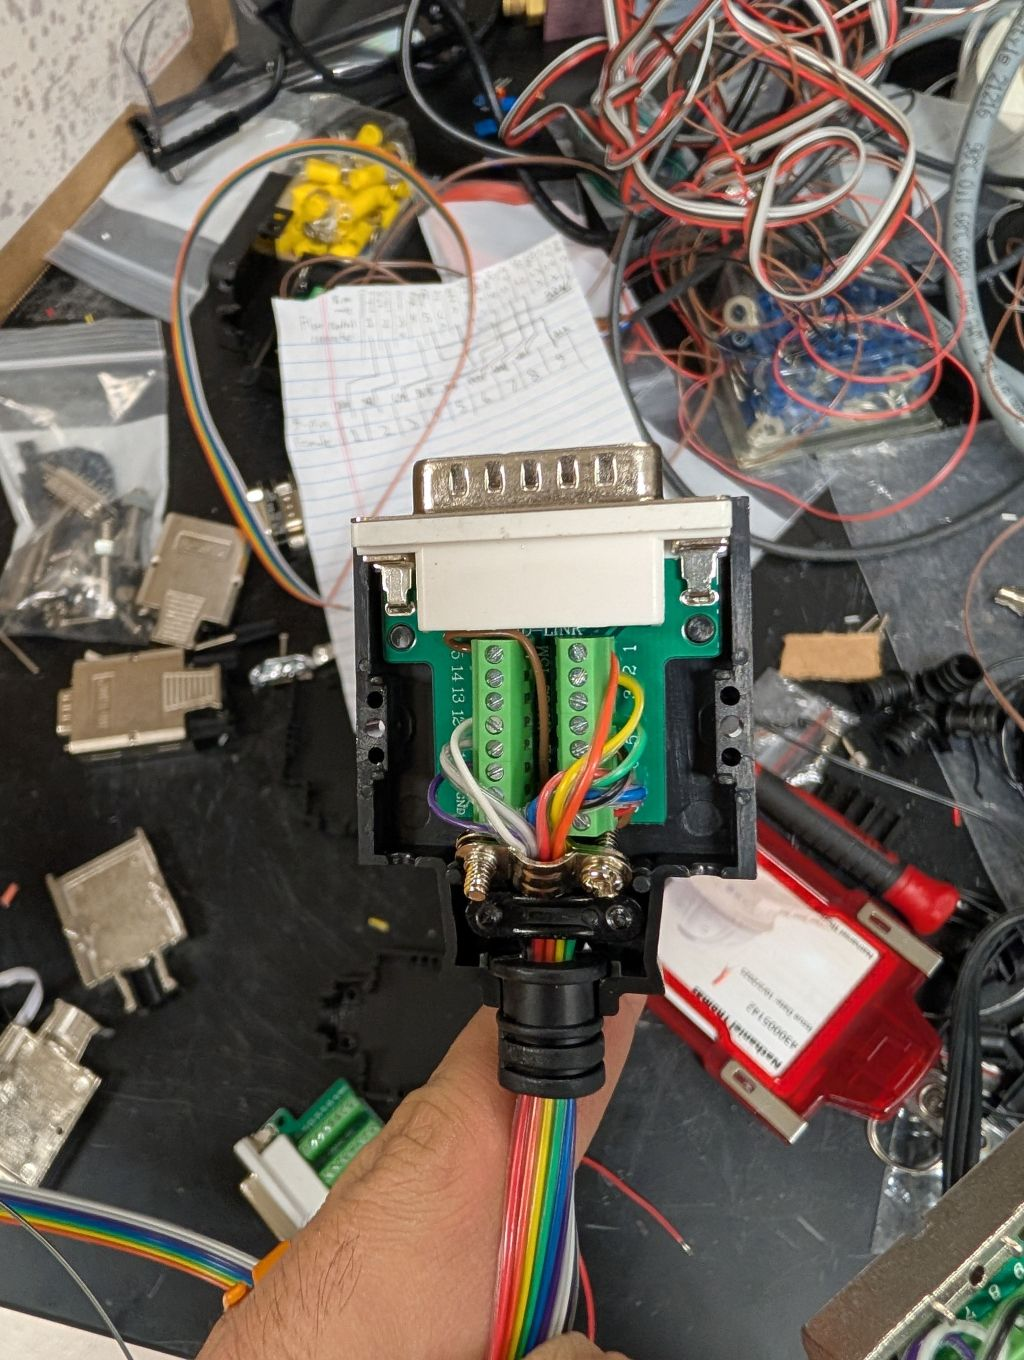
\includegraphics[width=0.3\textwidth]{./assets/pictures/gfc db15.jpg}
  \caption{Image of the wired DB15 connector for the Aalborg GFC17
  flow controllers.}
  \label{fig: gfc db15}
\end{figure}

\begin{figure}[H]
  \centering
  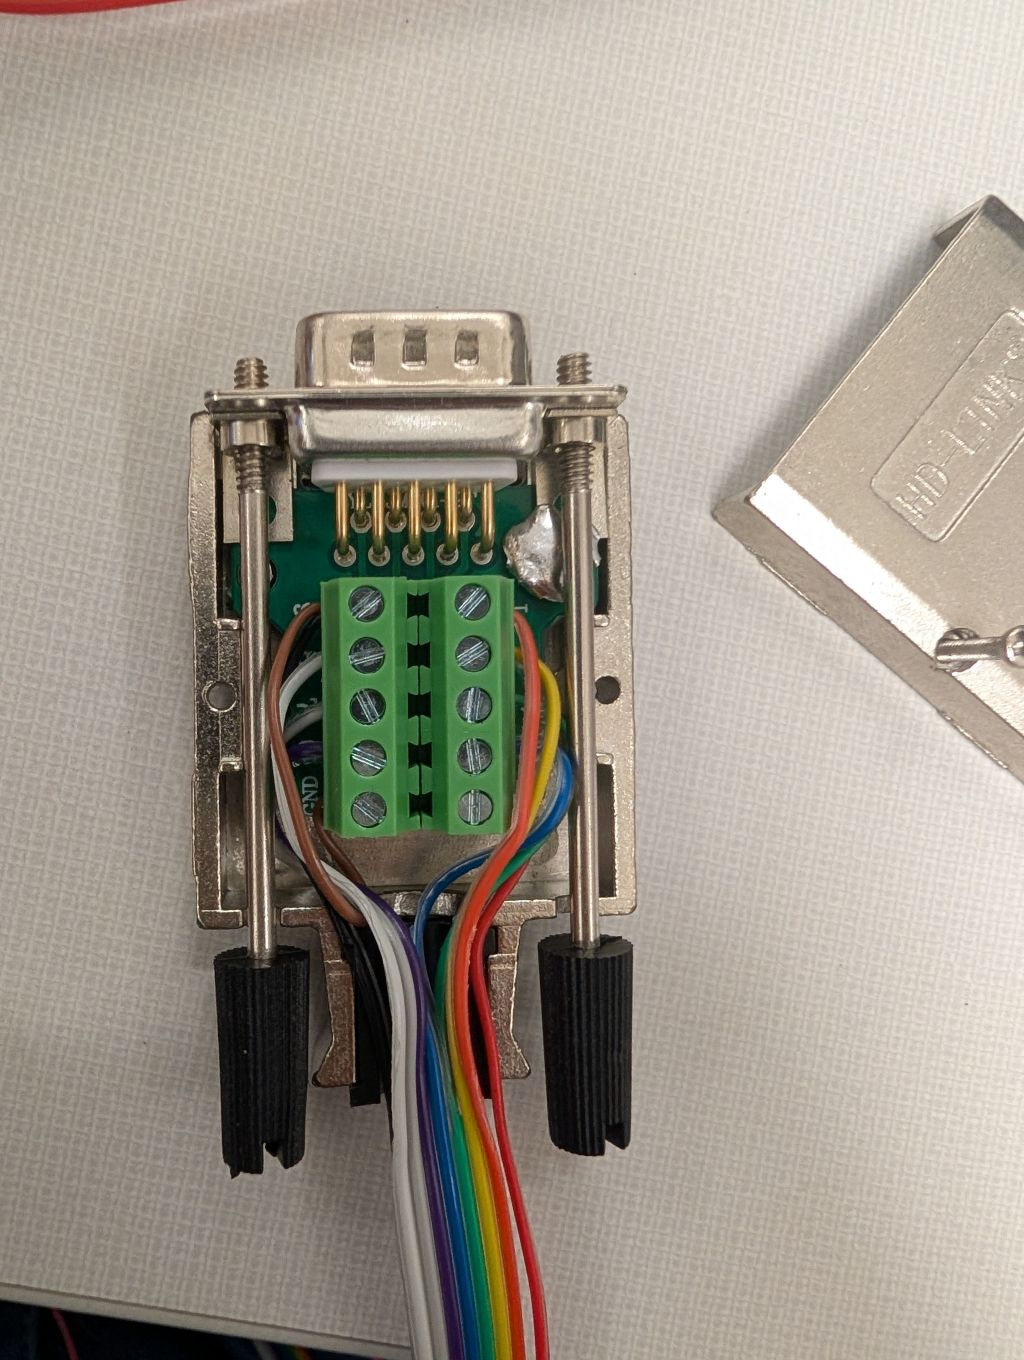
\includegraphics[width=0.3\textwidth]{./assets/pictures/gfc db9.jpg}
  \caption{Image of the wired DB9 connector for the Aalborg GFC17
  flow controllers.}
  \label{fig: gfc db9}
\end{figure}
